\documentclass{article}
\usepackage{arxiv}

\usepackage[utf8]{inputenc}
\usepackage[english, russian]{babel}
\usepackage[T1]{fontenc}
\usepackage{url}
\usepackage{booktabs}
\usepackage{amsfonts}
\usepackage{nicefrac}
\usepackage{microtype}
\usepackage{lipsum}
\usepackage{graphicx}
\usepackage{natbib}
\usepackage{doi}



\title{A template for the \emph{arxiv} style}

\author{ David S.~Hippocampus\thanks{Use footnote for providing further
		information about author (webpage, alternative
		address)---\emph{not} for acknowledging funding agencies.} \\
	Department of Computer Science\\
	Cranberry-Lemon University\\
	Pittsburgh, PA 15213 \\
	\texttt{hippo@cs.cranberry-lemon.edu} \\
	%% examples of more authors
	\And
	Elias D.~Striatum \\
	Department of Electrical Engineering\\
	Mount-Sheikh University\\
	Santa Narimana, Levand \\
	\texttt{stariate@ee.mount-sheikh.edu} \\
	%% \AND
	%% Coauthor \\
	%% Affiliation \\
	%% Address \\
	%% \texttt{email} \\
	%% \And
	%% Coauthor \\
	%% Affiliation \\
	%% Address \\
	%% \texttt{email} \\
	%% \And
	%% Coauthor \\
	%% Affiliation \\
	%% Address \\
	%% \texttt{email} \\
}
\date{}

\renewcommand{\shorttitle}{\textit{arXiv} Template}

%%% Add PDF metadata to help others organize their library
%%% Once the PDF is generated, you can check the metadata with
%%% $ pdfinfo template.pdf
\hypersetup{
pdftitle={A template for the arxiv style},
pdfsubject={q-bio.NC, q-bio.QM},
pdfauthor={David S.~Hippocampus, Elias D.~Striatum},
pdfkeywords={First keyword, Second keyword, More},
}

\begin{document}
\maketitle

\begin{abstract}
	Исследуется задача логической классификации с дискретными признаками. Предлагается метод ускорения синтеза монотонных логических корректоров, основанных на построении тупиковых корректных наборов элементарных классификаторов (ЭК) ранга 1. Ключевая проблема — вычислительная сложность поиска неприводимых покрытий булевой матрицы LK. Для её решения разработан алгоритм предварительной обработки: из матрицы удаляются охватывающие строки, что позволяет перейти к подматрице с упрощенной структурой и найти в ней неприводимые покрытия, формирующие корректные наборы. Корректность метода обоснована, а эксперименты подтвердили его эффективность, показав прирост скорости построения корректоров.
\end{abstract}


\keywords{First keyword \and Second keyword \and More}

\section{Introduction}

Задача классификации по прецедентам, или обучения с учителем, является одной из фундаментальных проблем в машинном обучении и анализе данных. Её целью является автоматическое отнесение новых объектов к одному из заранее известных классов на основе анализа конечного набора обучающих данных, для которых классовая принадлежность определена. Эффективные алгоритмы классификации критически важны в таких областях, как медицинская диагностика, прогнозирование редких событий, анализ финансовых рисков и обработка социологической информации, где от точности модели зависят принимаемые решения.

Для решения задач классификации, особенно в условиях недостатка статистических данных, успешно применяются логические (дискретные) методы. Фундамент для этих методов в России был заложен в работах С.В. Яблонского и Ю.И. Журавлева в 70–80-х годах прошлого века. Ранние подходы в рамках этого направления фокусировались на использовании элементарных классификаторов (ЭК) — простых правил вида «признак $x_j$ равен значению $\sigma$». Процесс классификации заключался в построении для каждого класса семейств таких корректных ЭК (не ошибающихся на обучающей выборке) и последующем процедуре голосования этих ЭК за классы для нового объекта.

Однако классические логические подходы сталкиваются с серьезными вычислительными и методическими трудностями. Когда признаки имеют множество допустимых значений, количество корректных ЭК становится чрезвычайно большим, при этом каждый из них может покрывать лишь малую часть прецедентов. Это приводит к двум ключевым проблемам: во-первых, возникают сложности с обеспечением общей корректности алгоритма, а во-вторых, процедура обучения требует решения сложных дискретных задач комбинаторной оптимизации, что вычислительно трудоемко.

Прорывом в преодолении этих ограничений стало развитие методов алгебро-логической коррекции, где корректность обеспечивается не отдельными ЭК, а их наборами. В данной работе предлагается усовершенствованный алгоритм построения таких наборов. Вместо работы с булевой матрицей $L_K$, число столбцов которой экспоненциально зависит от количества признаков, мы предлагаем альтернативный подход. Сначала строится компактная матрица сравнения с линейным числом столбцов, затем из неё удаляются избыточные (охватывающие) строки. На следующем этапе осуществляется переход к расширенной матрице и поиск в ней неприводимых покрытий, каждое из которых образует тупиковый монотонный корректный набор ЭК.

Предложенный метод позволяет значительно снизить вычислительную сложность этапа обучения по сравнению с традиционными подходами. В работе приведено теоретическое обоснование корректности алгоритма, доказывающее, что найденные наборы ЭК действительно обеспечивают безошибочную классификацию на обучающих данных. Проведенные вычислительные эксперименты подтвердили эффективность алгоритма, продемонстрировав его применимость для задач с большим числом признаков. Таким образом, основной вклад работы заключается в разработке более эффективной и масштабируемой процедуры синтеза логических классификаторов, которая решает ключевую проблему вычислительной трудоемкости, сохраняя при этом высокую точность.

\section{Headings: first level}
\label{sec:headings}

\lipsum[4] See Section \ref{sec:headings}.

\subsection{Headings: second level}
\lipsum[5]
\begin{equation}
	\xi _{ij}(t)=P(x_{t}=i,x_{t+1}=j|y,v,w;\theta)= {\frac {\alpha _{i}(t)a^{w_t}_{ij}\beta _{j}(t+1)b^{v_{t+1}}_{j}(y_{t+1})}{\sum _{i=1}^{N} \sum _{j=1}^{N} \alpha _{i}(t)a^{w_t}_{ij}\beta _{j}(t+1)b^{v_{t+1}}_{j}(y_{t+1})}}
\end{equation}

\subsubsection{Headings: third level}
\lipsum[6]

\paragraph{Paragraph}
\lipsum[7]



\section{Examples of citations, figures, tables, references}
\label{sec:others}

\subsection{Citations}
Citations use \verb+natbib+. The documentation may be found at
\begin{center}
	\url{http://mirrors.ctan.org/macros/latex/contrib/natbib/natnotes.pdf}
\end{center}

Here is an example usage of the two main commands (\verb+citet+ and \verb+citep+): Some people thought a thing \citep{kour2014real, hadash2018estimate} but other people thought something else \citep{kour2014fast}. Many people have speculated that if we knew exactly why \citet{kour2014fast} thought this\dots

\subsection{Figures}
\lipsum[10]
See Figure \ref{fig:fig1}. Here is how you add footnotes. \footnote{Sample of the first footnote.}
\lipsum[11]

\begin{figure}
	\centering
	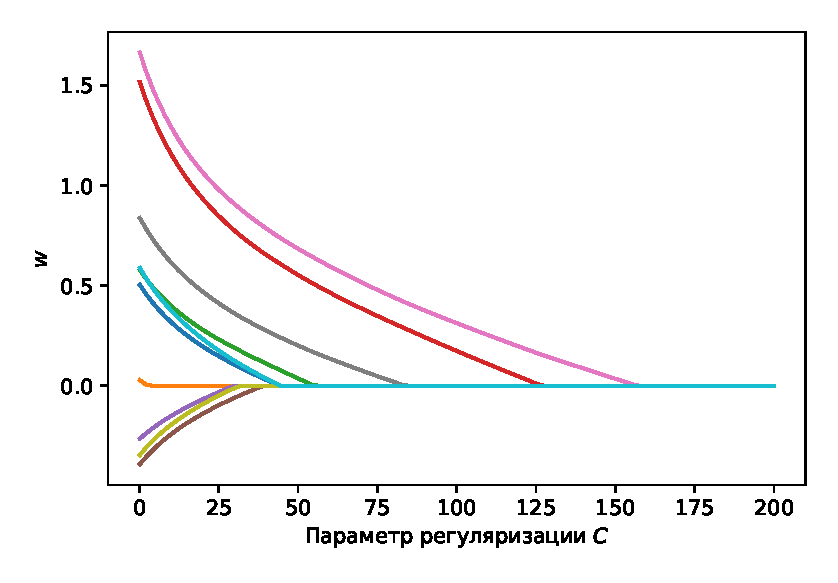
\includegraphics[width=0.5\textwidth]{../figures/log_reg_cs_exp.eps}
	\caption{Sample figure caption.}
	\label{fig:fig1}
\end{figure}

\subsection{Tables}
See awesome Table~\ref{tab:table}.

The documentation for \verb+booktabs+ (`Publication quality tables in LaTeX') is available from:
\begin{center}
	\url{https://www.ctan.org/pkg/booktabs}
\end{center}


\begin{table}
	\caption{Sample table title}
	\centering
	\begin{tabular}{lll}
		\toprule
		\multicolumn{2}{c}{Part}                   \\
		\cmidrule(r){1-2}
		Name     & Description     & Size ($\mu$m) \\
		\midrule
		Dendrite & Input terminal  & $\sim$100     \\
		Axon     & Output terminal & $\sim$10      \\
		Soma     & Cell body       & up to $10^6$  \\
		\bottomrule
	\end{tabular}
	\label{tab:table}
\end{table}

\subsection{Lists}
\begin{itemize}
	\item Lorem ipsum dolor sit amet
	\item consectetur adipiscing elit.
	\item Aliquam dignissim blandit est, in dictum tortor gravida eget. In ac rutrum magna.
\end{itemize}


\bibliographystyle{unsrtnat}
\bibliography{references}

\end{document}